\section{Moduli Theory}
\subsection{Introduction and Motivation}
The goal of a moduli problem is to classify a collection of geometric objects upto some sort of equivalence.
The \textit{geometric object} can vary significantly from one moduli problem to another. 
For example, in the rest of this thesis we will majorly be dealing with two moduli problems - one where the object in consideration is a rational plane curve, and the other where the rational plane curve comes together with its embedding $\mu$ in $\mathbb{P}^{r}$.

Before I what exactly a Moduli problem entails, consider the following example:

\begin{example}
    \label{exLinesInPlane}
\begin{align*}
    \mathcal{X} = \{\{(x, ax + b) \in \mathbb{R}^{2}: x \in \mathbb{R}\} : (a,b) \in \mathbb{R}^{2}\}
\end{align*}
Each object in this set $\mathcal{X}$ is a line given by the equation $y = ax + b$.
Notice that this set $\mathcal{X}$ is parameterised by points in $\mathbb{R}^{2}$, that is, we have a map $\varphi: \mathcal{X} \to \mathbb{R}^{2}$, which sends the line $y = ax + b$ to $(a,b)$.  
Therefore, we can think of the family of nonvertical lines in $\mathbb{R}^{2}$ as the map:
\[\begin{tikzcd}
	{\mathcal{X}} \\
	\\
	{\mathbb{R}^2}
	\arrow["\varphi",from=1-1, to=3-1]
\end{tikzcd}\]
With the fibre $\varphi^{-1}(p)$ over the point $p = (a,b)$ being the line $y = ax + b$.
An advantage of describing the set of lines $\mathcal{X}$ with this parameterisation is that points close to each other in $\mathbb{R}^{2}$ correspond to lines which are ``close to each other".  

\end{example}

This example motivates the definition of a family: 
\begin{definition}
    A morphism $\mathcal{X} \to B$ between schemes (with possibly additional structure) will be referred to as a family over the scheme $B$. This will often be denoted as $\mathcal{X}/B$.
\end{definition}
The fibres over points of the scheme $B$ correspond to out geometric objects, in context of example \ref{exLinesInPlane} the fibres were non-vertical lines in $\mathbb{R}^{2}$.
\par It's usually easier to deal with families when we define a notion of equivalent families. 
That is, an equivalence relation on the set of families, $S(B)$, over the scheme $B$. 
Since we are dealing with schemes, an obvious notion of equivalence between families $\mathcal{X}/B$ and $\mathcal{X}'/B$ can be defined with isomorphisms. That is, an isomorphism, $\psi: \mathcal{X} \to \mathcal{X}'$ such that the following diagram commutes:
\[
\begin{tikzcd}
    {\mathcal{X}} && {\mathcal{X}'}\\
    \\
                  & {B} 
     \arrow["\psi", from = 1-1, to = 1-3]
     \arrow[from = 1-1, to = 3-2]
     \arrow[from = 1-3, to = 3-2]
\end{tikzcd}
\]
Note that isomorphisms over the scheme $B$ is just an example of an equivalence relation on $S(B)$, over the rest of the thesis we will encounter different equivalence realtions which are appropriate for the given situations.
When two families $\mathcal{X}/B$ and $\mathcal{N}/B$ lie in the same equivalence class in $S(B)$, we write $\mathcal{X}/B \simeq \mathcal{N}/B$.
\par Finally, a moduli problem consists of:
\begin{itemize}
    \item A class of geometric objects.
    \item A family of these geometric objects over a parameter space (base scheme).
    \item And an equivalence relation on the set of families, $S(B)$, over a base $B$.
\end{itemize}

An important idea while dealing with families of objects is being able to change your base space.
If we have a family $\mathcal{X}/B$ and a morphism $\varphi: B' \to B$ then one can define a new family over the base $B'$ given by the fibre product $\mathcal{X} \times_{B} B' \to B'$.
\[
\begin{tikzcd}
    {\varphi^{*}\mathcal{X} := \mathcal{X} \times_{B} B'} & & \mathcal{X}\\
    \\
    B' && B
    \arrow[ from = 1-3, to = 3-3]
    \arrow[from = 1-1, to = 1-3]
    \arrow["\varphi", from = 3-1, to = 3-3]
    \arrow[from = 1-1, to = 3-1]
\end{tikzcd}
\]
The family $\varphi^{*}\mathcal{X}/B'$ is called the pullback family of $\mathcal{X}/B$ along the morphism $\varphi$.
For our families to behave ``nicely" we would like pullbacks to commute with equivalence. 
That is, if $\mathcal{X}/B \simeq \mathcal{N}/B $ and $\varphi B' \to B$ is a morphism then we would like:
\begin{align*}
    \varphi^{*}\mathcal{X}/B' \simeq \varphi^{*}\mathcal{N}/B'.
\end{align*}

Before we formally define a moduli problem in the context of categories let's look at example \ref{exLinesInPlane} carefully.
\begin{example}
    \label{compExLinesInplane}
    In example \ref{exLinesInPlane} we defined a parameter space for non-vertical lines in $\mathbb{R}^{2}$. 
    But we would like to define a parameter/base space such that we can characterize all lines (including vertical ones) in $\mathbb{R}^{2}$.
    \par In the diagram above we have embedded $\mathbb{R}^{2}$ in $\mathbb{R}^{3}$ as the plane $z = 1$.
    For each line $ax + by + c = 0 $, there exists a plane, $L := ax + by + cz = 0$,  through the origin in $\mathbb{R}^{3}$ such that $L \cap \{z=1\}$ corresponds to the line $ax + by + c = 0 $.
    \par We also know that each plane through the origin, $\mathbb{R}^{3}$, corresponds to a line through the origin (its normal vector). 
    This gives a bijection between the set of lines in $\mathbb{R}^{2}$ and the points of $\mathbb{RP}^{2}\backslash \{ [0:0:1]\}$, which can be seen as the family:
    \[
        \begin{tikzcd}
            \mathcal{Y} := \{\text{set of lines in } \mathbb{R}^{2}\}\\
            \\
            \mathbb{RP}^{2}\backslash {[0:0:1]}
            \arrow["\psi", from = 1-1, to = 3-1]
        \end{tikzcd}
    \]
    Notice that we are one point away from our parameter space being the entire projective space $\mathbb{RP}^{2}$.
    It's natural to ask what space does $\mathbb{RP}^{2}$ parameterise?
    Luckily the answer to this question is quite striaghtforward.
    We have a bijection between lines in $\mathbb{RP}^{2}$ and points in $\mathbb{RP}^{2}$ given by:
    \[
        \begin{tikzcd}
            {\mathbb{RP}^{2}} & & {\{\text{lines in }\mathbb{RP}^{2}\}} \\
            {[a:b:c]} \arrow[u, phantom, sloped, "\in"]& & {\{[x:y:z] \in \mathbb{RP}^{2}: ax + by + cz = 0 \}}\arrow[u, phantom, sloped, "\in"].
            \arrow["\gamma", leftarrow, from = 1-1, to = 1-3]
            \arrow[ leftrightarrow, from = 2-1, to = 2-3]
            %\arrow[phantom, from = 2-1, to = 1-1, sloped, "\in"]
            %\arrow[phantom, from = 2-2, to = 1-2, sloped, "\in"]
        \end{tikzcd}
    \]
    And this can be seen as a family $\gamma : \mathbb{RP}^{2}\to \mathbb{RP}^{2}$ of lines in $\mathbb{RP}^{2}$.
    \par We can now interpret the families $\mathcal{X}/\mathbb{R}^{2}$ (example \ref{exLinesInPlane}) and $\mathcal{Y}/\{\mathbb{RP}^{2}\backslash {[0:0:1]}\} $ as families of lines in $\mathbb{RP}^{2}$ by embedding $\mathbb{R}^{2}$ in $\mathbb{RP}^{2}$, giving us the three families:
    \begin{itemize}
        \item $\varphi : \mathcal{X} \to \mathbb{R}^{2}$
    \item $\psi: \mathcal{Y} \to \mathbb{RP}^{2}\backslash {[0:0:1]}\} $
    \item $\gamma: \mathbb{RP}^{2} \to \mathbb{RP}^{2}$.
\end{itemize}
For the inclusion maps, 
\begin{itemize}
    \item $i: \mathbb{R}^{2}\hookrightarrow \mathbb{RP}^{2}$,
\item $j: \mathbb{RP}^{2}\backslash {[0:0:1]}\} \hookrightarrow \mathbb{RP}^{2}$,
\end{itemize}
we have: 
\begin{align*}
    i^{*}\mathbb{RP}^{2} \simeq &\mathcal{X}\\
    j^{*}\mathbb{RP}^{2} \simeq &\mathcal{Y}.
\end{align*}
Further, for any family of lines in $\mathbb{RP}^{2}$, $\mathcal{Z}/B$, there exists a unique morphism $\phi :B \to \mathbb{RP}^{2}$, such that $\mathcal{Z}/B$ is equivalent to the pullback family along $\phi$.
We will see that the family $\gamma: \mathbb{RP}^{2} \to \mathbb{RP}^{2}$ satisfies the properties of a \textbf{universal family}, with the base space being defined as a \textbf{fine moduli space}.
\end{example}

\begin{definition}[Fine moduli spaces]
    A \textbf{universal family} for a moduli problem is a family $U/M$ such that for any other family $\mathcal{X}/B$ there exists a unique morphism $\varphi: B \to M$ with the property that $\varphi^{*}U \simeq \mathcal{X}$.
    \par The base space of the universal family $M$ is called a \textbf{fine moduli space}. The morphism $\varphi$ is called the \textbf{classifying map} of the family $\mathcal{X}/B$.
\end{definition}

\subsection{Moduli Problems in the language of Categories}
The properties of a moduli problem, like commutativity of pullback families with equivalences, can be stated elegantly in the language of categories.
To see this, consider the following commutative diagram:
\[
    \begin{tikzcd}
        {\varphi^{*}\mathcal{X} := \mathcal{X} \times_{B} B'} & & \mathcal{X}\\
        \\
        B' && B
        \arrow[ from = 1-3, to = 3-3]
        \arrow[from = 1-1, to = 1-3]
        \arrow["\varphi", from = 3-1, to = 3-3]
        \arrow[from = 1-1, to = 3-1]
    \end{tikzcd}
\]
Given a morphism $\varphi: B' \to B$ we get a map from $S(B)$ to $S(B')$ which sends $\mathcal{X}/B$ to $\varphi^{*}\mathcal{X}/B'$. 
Remember that $S(B)$ denotes the equivalence class of families over $B$ - hence ensuring that pullback is defined upto equivalence.
We can interpret this reversing of directions as a contravariant functor which sends each scheme to the equivalence class of families over it. 
Consider a functor $S$ defined as:
\begin{align*}
    S:\textbf{Sch}^{op} & \to \textbf{Sets}\\
    X &\mapsto S(X):=\{\text{Equivalence classes of families over }X\},
\end{align*}
where for $\varphi \in \text{Mor}(A,B)$, $S(\varphi) = \varphi^{*} \in \text{Mor}(S(B),S(A))$. 
\subsubsection{Representable Funtors and Fine Moduli Spaces}
\begin{definition}[Functor of Points]
    For any scheme $X$ there exists a contravariant set-valued functor, $h_{X}$, called its \textbf{funtor of points}.
    This funtor is defined as: 
    \begin{align*}
        h_{X}: \textbf{Sch}^{op} &\to \textbf{Sets}\\
        B &\mapsto \emph{Hom}(B,X),
    \end{align*}
    where for $\varphi:B' \to B$, $h_{X}(\varphi)$ is defined as:
    \begin{align*}
        h_Y(\varphi):\emph{Hom}(B,X) &\to \emph{Hom}(B',Y)\\
        \beta &\mapsto \beta \circ \varphi
    \end{align*}
\end{definition}
\begin{definition}[Representable Functors]
    A functor $S$ isomorphic to a functor points (for some scheme $X$) is called a \textbf{representable functor}.
    If $\mathcal{U}:h_{Y}\to S$ is an isomrphism of functors, then we say that the pair $(Y, \mathcal{U})$ represents $S$.
\end{definition}
By Yoneda's Lemma (appendix) we knoww that we can identify the natiral transformation $\mathcal{U}:h_{Y}\to S$ with an element of $S(Y)$.
Suppose the element of $S(Y)$ corresponding to $\mathcal{U}$ is $U$.
Then $(Y,U)$ is said to represent $S$.
\begin{proposition}
    A family $U/M$ is the universal family (with M the fine moduli space) for a moduli problem, if and only if the pair $(M,U)$ represents the moduli functor $S$.
\end{proposition}
\begin{proof}
    \textit{Suppose $(M,U)$ represents the moduli functor $F$}.
    \par Then there exists an isomorphism of functors:
    \begin{align*}
        \mathcal{U}:h_{M} \to F,
    \end{align*}
    which at the level of objects maps in the following manner:
    \begin{align*}
        \mathcal{U}_{M}:h_{M}(M) &\to F(M)\\
        \text{id}_{M} &\mapsto U/M.
    \end{align*}
    Let $\mathcal{V}:= \mathcal{U}^{-1}$ be the inverse functor. Now consider any $\varphi: B \to M$, we have the commutative diagram:
    \[
        \begin{tikzcd}
            h_{M}(M) & & F(M) & & h_{M}(M)\\
            h_{M}(B) & & F(B) & & h_{M}(B)
            \arrow["\mathcal{U}_{M}", from = 1-1, to = 1-3]
            \arrow["\mathcal{V}_{M}", from = 1-3, to = 1-5]
            \arrow["\mathcal{U}_{B}", from = 2-1, to = 2-3]
            \arrow["\mathcal{V}_B", from = 2-3, to = 2-5]
            \arrow["F(\varphi)", from = 1-3, to = 2-3]
            \arrow["\_\circ \varphi", from = 1-1, to = 2-1]
            \arrow["\_\circ \varphi", from = 1-5, to = 2-5]
        \end{tikzcd}
    \]
    Since $\mathcal{U}$ is an isomorphism $\mathcal{U}_{B}$ is a bijection for all $B$. Implying that for all $\mathfrak{X}/B \in F(B)$ there exists $\varphi_{\mathfrak{X}}\in h_{M}(B)$ such that $\mathcal{U}_{B}(\varphi_{\mathfrak{X}}) = \mathfrak{X}/B$. 
    For this morphism, $\varphi_{\mathfrak{X}}$, consider the following diagram (with the element being chased on the right).
    \[
        \begin{tikzcd}
            h_{M}(M) & & F(M) & & \text{id}_{M} && U/M\\
            h_{M}(B) & & F(B) & & \varphi_{\mathfrak{X}} && \mathfrak{X}/B = F(\varphi_{\mathfrak{X}})(U/M) = \varphi_{\mathfrak{X}}^{*}U/B
            \arrow["\mathcal{U}_{M}", from = 1-1, to = 1-3]
            \arrow["\mathcal{U}_{B}", from = 2-1, to = 2-3]
            \arrow["F(\varphi_{\mathfrak{X}})", from = 1-3, to = 2-3]
            \arrow["\_\circ \varphi_{\mathfrak{X}}", from = 1-1, to = 2-1]
            \arrow["\mathcal{U}_{M}", mapsto, from = 1-5, to = 1-7]
            \arrow["\mathcal{U}_{B}", mapsto, from = 2-5, to = 2-7]
            \arrow["\_\circ \varphi_{\mathfrak{X}}", mapsto, from = 1-5, to = 2-5]
            \arrow["F(\varphi_{\mathfrak{X}})", mapsto, from = 1-7, to = 2-7]
        \end{tikzcd}
    \]
    Via commutativity of the above diagram it follows that $\mathfrak{X}/B = \varphi_{\mathfrak{X}}^{*}U/B$. 
    The classifying map, $\varphi_{\mathfrak{X}}$, is unique since the $\mathcal{U}_{B}$ is a bijection. 
    Hence, we have proved one direction of the hypothesis.
    \par \textit{Suppose $U/M$ is a universal family}.
    \par We need to show that the naturam transformation $\mathcal{U}:h_{M} \to F$, which corresponds to $U/M \in F(M)$ (via the bijection from Yoneda's lemma), is an isomorphism of functors.
    Recall that a natural transformation, $\mathcal{U}$, is an isomorphism if for a each $B \in \textbf{Sch}$ the induced map $\mathcal{U}_{B}$ is a set theoretic bijection. 
    We showed above that for any $\varphi \in h_{M}(B)$, $\mathcal{U}_{B}(\varphi) = \varphi^{*}U/B$: 
    \begin{align*}
        \mathcal{U}_{B}: h_{M}(B) = \text{Hom}(B,M) &\to F(B) \\
        \varphi &\mapsto \varphi^{*}U/B.
    \end{align*}
    Further, via the universal propety of $U/M$, for each family $\mathfrak{X}/B$ there exists a unique morphism (the classifying map) $\varphi_{\mathfrak{X}} \in h_{M}(B)$. 
    Let this correspondence between families over $B$ and morphisms in $\text{Hom}(B,M)$ by a map $L$. Then,
    \begin{align*}
        L \circ \mathcal{U}_{B} (\varphi) &= L(\varphi^{*}U/B) = \varphi \\
        \mathcal{U}_{B} \circ L (\mathfrak{X}/B) &= \mathcal{U}_{B} (\varphi_{\mathfrak{X}}) = \varphi^{*}_{\mathfrak{X}} U/M = \mathfrak{X}/B .
    \end{align*}
    Therefore, $\mathcal{U}_{B}$ is a bijection for all $B \in \textbf{Sch}$, proving that $\mathcal{U}$ is an isomorphism of functors.
\end{proof}

\subsubsection{Coarse Moduli Spaces}

Notice that the previous proposition doesn't deal with the existence of fine moduli spaces in general.
There are many interesting moduli functors (one which we will encounter later) in the thesis which aren't representable.
That is, fine moduli spaces need not exist for such moduli problems.
It's now natural to ask if there is a way we can relax the definition of a fine moduli space to construct some sort of a \textit{best approximation}? We will call this approximation the \textbf{coarse moduli space}.

\begin{definition}
    A \textbf{coarse moduli space} for a moduli functor $S$ is the pair $(M, \mathcal{V})$, where $M$ is a scheme and $\mathcal{V}:S \to h_{M}$ is a natural transform of functor such that:
    \begin{itemize}
        \item $(M,\mathcal{V})$ is initial across all such pairs,
        \item The map between sets, 
            \begin{align*}
                \mathcal{V}_{\emph{Spec}\mathbb{C}}: S(\emph{Spec}\mathbb{C}) \to \emph{Hom}(\emph{Spec}\mathbb{C}, M),
            \end{align*}
            is a bijection.
    \end{itemize}
\end{definition}
\subsection{Families of Points in $\mathbb{P}^{1}$}
In this section we will look at families of distint point in $\mathbb{P}^{1}$. 
This example will serve as an important building block for the study of moduli spaces of marked rational plane curves. 
For the rest of this section we denote with $x$, the point $[x:1] \in \mathbb{P}^{1}$, and $\infty$ for the point $[0:1]$.
\par By a family of $n$ points in $\mathbb{P}^{1}$ over a scheme $B$ we mean a diagram:
\[
    \begin{tikzcd}
        B \times \mathbb{P}^{1}\\
        \\
        B
        \arrow["\pi",xshift = -2ex, from = 1-1, to = 3-1]
        \arrow[ xshift = 1ex,from = 3-1, to = 1-1]
        \arrow[ xshift = 2.3ex,from = 3-1, to = 1-1]
        \arrow[ swap, "\sigma_{i}", xshift = 3.6ex,from = 3-1, to = 1-1]
    \end{tikzcd}
\]
Where $\sigma_{i}$ are disjoint sections. Therefore for each $b \in B$ we get $n$ points in $\mathbb{P}^{1}$ given by the $n$ sections. 
\par For the rest of this section we are interested in the case where $n \geq 4$, since for any three distinct points, $p_{1}, p_{2}, p_{3}$, there exists an automorphism of $\mathbb{P}^{1}$ which sends them to $0,\,1,\text{ and }\infty$ respectively - implying all tuples of three or less points are equivalent.

\subsubsection{Projective Equivalence of Families}
Two families of $n$-points over a scheme $B$ are said to be projectively equivalent if there exists an automorphism $\phi \in \text{Aut}(\mathbb{P}^{1})$ such that the diagram:
\[
    \begin{tikzcd}
        B \times \mathbb{P}^{1} & & B \times \mathbb{P}^{1}\\
                                & & \\
        B & & B
        \arrow["\pi",xshift = -2ex, from = 1-1, to = 3-1]
        \arrow[ swap, "\sigma_{i}", xshift = 1.2ex,from = 3-1, to = 1-1]
        \arrow["\pi",xshift = -2ex, from = 1-3, to = 3-3]
        \arrow[ swap, "\sigma_{i}'", xshift = 1.2ex,from = 3-3, to = 1-3]
        \arrow["\text{id}\times \phi", from = 1-1, to = 1-3]
        \arrow[equal,  from = 3-1, to= 3-3]
    \end{tikzcd}
\]
commutes.

\subsubsection{Family of 4 points - Quadruples}
Define $Q:= \mathbb{P}^{1} \times \mathbb{P}^{1} \times \mathbb{P}^{1} \times \mathbb{P}^{1} \backslash \{\text{diagonals}\}$. 
Then for any family of four points over a scheme $B$ we have a map $\sigma: B \to Q$ where each coordinate is defined by the section $\sigma_{i}$.
This map $\sigma$ acts as the classifying map, and shows that $Q$ is a fine moduli space for families of four points and the universal family is of the form:
\[
    \begin{tikzcd}
        Q \times \mathbb{P}^{1}\\
        \\
        Q
        \arrow["\pi",xshift = -2ex, from = 1-1, to = 3-1]
        \arrow[ xshift = 1ex,from = 3-1, to = 1-1]
        \arrow[ xshift = 2.3ex,from = 3-1, to = 1-1]
        \arrow[ xshift = 3.6ex,from = 3-1, to = 1-1]
        \arrow[ swap, "\sigma_{i}", xshift = 4.9ex,from = 3-1, to = 1-1]
    \end{tikzcd}
\]
with $\sigma_{i}(\textbf{p}) = (\textbf{p},p_{i})$.
\par Now we want to take into consideration the notion of projective equivalence. 
Remember that any three points $p_{1},\, p_{2}, \,p_{3}$ define an automorphism $\alpha$ of $\mathbb{P}^{1}$ which sends them to $0,\,1\,\text{and }\infty$.
For a quedrupule of points $p_1, \dots, p_4$, let $\alpha$ be the automorphism determined by the first three points. 
Then we define the \textbf{cross ratio} of the quadruple as $\alpha(p_{4}) \in \mathbb{P}^{1}\backslash\{0,1,\infty\}$.
\par It follows that each quadruple $(p_{1}, \dots, p_{4})$ is projctively equivalent to $(0,1,\infty,q)$ where $q$ is the cross ratio of the quadruple. Consquently we have a bijection:
\begin{align*}
    \mathcal{M}_{0,4} := \{\text{Equivalence class of quadruples}\} \leftrightarrow \mathbb{P}^{1}\backslash\{0,1,\infty\}.
\end{align*}
It's easy to show that $\mathcal{M}_{0,4}$ is the \textbf{fine moduli space} for families of quadruples with the universal family given by:
\[
    \begin{tikzcd}
        \mathcal{M}_{0,4} \times \mathbb{P}^{1}\\
        \\
        \mathcal{M}_{0,4},
        \arrow["\pi",xshift = -2ex, from = 1-1, to = 3-1]
        \arrow[ xshift = 1ex,from = 3-1, to = 1-1]
        \arrow[ xshift = 2.3ex,from = 3-1, to = 1-1]
        \arrow[ xshift = 3.6ex,from = 3-1, to = 1-1]
        \arrow[ swap, "\tau_{i}", xshift = 4.9ex,from = 3-1, to = 1-1]
    \end{tikzcd}
\]
where $\tau_1 :=0$, $\tau_2 :=1$, $\tau_3 := \infty$, $\tau_4(p) = p$.

\subsubsection{Family of n-points}
For a quadruples of points $(p_{1}, p_{2}, p_{3}, p_{4})$ let $\lambda((p_{1}, p_{2}, p_{3}, p_{4}))$ denote their cross ratio.
Then we can sharacterize projective equivalence of two $n$-tuples in the following manner.
Let $(p_{1}, p_{2}, p_{3},\dots,p_{n})$ and $(p'_{1}, p'_{2}, p'_{3},\dots,p'_{n})$ be two $n$-tuples; they are said to be projectively equivalent if and only if for all $i\geq 4$:
\begin{align*}
     \lambda(p_{1}, p_{2}, p_{3}, p_{i}) = \lambda(p'_{1}, p'_{2}, p'_{3}, p'_{i}).
\end{align*}
With this characterisation it's easy to see that:
\begin{align*}
    \mathcal{M}_{0,n} \simeq \mathcal{M}_{0,4} \times \dots \times \mathcal{M}_{0,4} \backslash\{diagonals\},
\end{align*}
where the product has $n-3$ elements.

\section{Stable n-pointed Curves}
For the rest of this thesis, a rational plane curve (or a plane curve) will refer to a one dimensional variety that's birational to $\mathbb{P}^{1}$. 
In this section we will look at moduli spaces of plane curves with $n$-marked points.
This will help us in building intution for understanding the moduli space of stable maps, which we will use to prove Kontsevich's forumla.
A plane curve, C, with $n$ distinct point $p_{1},\dots, p_{n} \in C$ will be called a $n$-pointed rational curve, and will be denoted by the tuple $(C, p_{1}, \dots, p_{n})$.

\subsection{Families of smooth $n$-pointed curves}
\begin{definition}
    A family of $n$-pointed rational plane curves is a flat and proper morphism of schemes $\pi: X \to B$, such that the geometric fibres $\pi^{-1}(b)$ for all $b \in B$ are projective rational curves.
    Further, this morphism is equipped with $n$ disjoint sections $\sigma_{i}:B \to X$ which represent the $n$ marked points on each fibre.
\end{definition}
An equivalence between two families $\pi: \mathfrak{X} \to B$ and $\pi': \mathfrak{X}' \to B$ is an isomorphism $\phi: \mathfrak{X} \to \mathfrak{X}'$ such that the following diagram commutes:
\[
    \begin{tikzcd}
        \mathfrak{X} & & \mathfrak{X}'\\
                                & & \\
        B & & B
        \arrow[swap, "\pi",xshift = -1ex, from = 1-1, to = 3-1]
        \arrow[ swap, "\sigma_{i}", xshift = 1ex,from = 3-1, to = 1-1]
        \arrow[swap, "\pi",xshift = -1ex, from = 1-3, to = 3-3]
        \arrow[ swap, "\sigma_{i}'", xshift = 1ex,from = 3-3, to = 1-3]
        \arrow["\phi", from = 1-1, to = 1-3]
        \arrow[equal,  from = 3-1, to= 3-3]
    \end{tikzcd}
\]
For families, $\mathfrak{X}/B$ where the geomteric fibres are \textit{isomorphic} to $\mathbb{P}^{1}$:
\begin{itemize}
    \item If $n=1$ then $\mathfrak{X} \simeq \mathbb{P}(\varepsilon)$, where $\varepsilon$ is a rank 2 vector bundle on $B$.
    \item For $n=2$ this vector bundle splits.
    \item And for $n\geq 3$ there is a unique isomorphism $\mathfrak{X}\to B \times \mathbb{P}^{1}$. 
        Which makes this case equivalent to classification of families of $n$ points on $\mathbb{P}^{1}$ upto projective equivalence.
\end{itemize}
From the third point above it follows that, for $n\geq 4$, there exists a fine moduli space $\mathcal{M}_{0,n}$ for the problem of classifying $n$-pointed \textit{smooth} rational curves up to isomorphism.
We have seen that for $n=3$, $\mathcal{M}_{0,3}$ is a single point space, hence are first interesting example is $\mathcal{M}_{0,4}$ which can be interpreted as $\mathbb{P}^{1}\backslash\{0,1,\infty\}$.

\subsection{$\mathcal{M}_{0,4}$ and Compactification of $\mathcal{M}_{0,n}$}
When we see $\mathcal{M}_{0,4}$ as the projective line minus three points it's clear that it is not a compact space.
In general, for a good intersection theory to exist on our moduli space, it is necessary for them to be compact. 

\begin{example}
    \label{M04Example}
    We look at the universal family over $\mathcal{M}_{0,4}$ and see what happens when we compactify it to $\mathbb{P}^{1}$. 
    As discussed in the previous section, the universal family is $\pi :\mathcal{M}_{0,4} \times \mathbb{P}^{1} \to \mathcal{M}_{0,4}$, with sections $\tau_1 :=0$, $\tau_2 :=1$, $\tau_3 := \infty$, $\tau_4(p) = p$.
    This can be visualised as the following diagram, where $U_{q} = \pi^{-1}(q)$
    \begin{center}
    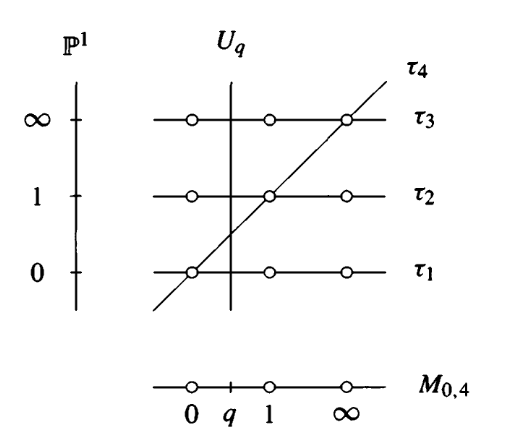
\includegraphics[scale = 0.3]{Chapters/Images/M_04_UniversalFam.png}
    \end{center}
    If we compactify $\mathcal{M}_{0,4}$ to $\mathbb{P}^{1}$ then the sections will no longer be disjoint.
    The diagnoal section $\tau_{4}$ will intersect the other $\tau_{i}'$s at $0,\,1\,\text{and }\infty$ respectively. 
    Therefore, the geometric sections over the points $0,\,1,\, \text{and }\infty$ are $3$-pointed curves, rather than $4$ pointed ones.
    \par To fix this problem we can blow up the universal family $\mathbb{P}^{1} \times \mathbb{P}^{1}$ at the three points, $\tau_{4}\cap \tau_{i}$, for $1\leq i \leq 3$.
    This process of blowing replaces each point $\tau_{4}\cap \tau_{i}$ with a copy of $\mathbb{P}^{1}$ (the exceptional divisor).
    Let $\tilde{\tau}_{i}$ denote the sections to the the blowup of the unversal family, then the fibre over $0$, $U_{0}$, looks like the following.
    \begin{center}
    \begin{tikzpicture}
        \draw (1,0) -- (1,4);
        \draw (0,1) -- (4,0);
    \draw[Circle-Circle] (1,3) node[right] {$\tilde{\tau}_{3}(0)$} -- (1,2)node[right] {$\tilde{\tau}_{2}(0)$};
        \draw[Circle-Circle] (2,0.5)node[below] {$\tilde{\tau}_{1}(0)$} -- (3,0.25)node[below] {$\tilde{\tau}_{4}(0)$};
    \end{tikzpicture}    
    \end{center}
    This fibre clearly isn't a smooth variety isomorphic to $\mathbb{P}^{1}$, but it gives us an idea of curves we may want to include in our family if we want our moduli space to be compact. 
    To be specific, we will include reducible curves with some additional structures in our family.
\end{example}
Taking the preceeding example as motivation we introduce the notion of \textit{trees} and \textit{stable curves}.
\begin{definition}
    A \textbf{tree of projective lines} is a connected curve such that:
    \begin{itemize}
        \item All irreducible components are isomorphic to $\mathbb{P}^{1}$.
        \item The points of intersection between irreducible components are ordinary double points (so no intersections are tangential).
        \item There are no closed cricuits, that is, if a node is removed, then the curve becomes disconnected.
    \end{itemize}
    We will refer to these as just trees.
    Further, the irreducible components are called \textbf{twigs}.
\end{definition}
\begin{definition}
    Let $n  \geq 3$. 
    We refer to the marked points and nodes as \textit{special points}.
    A stable $n$-pointed rational curve is a tree $C$ of projective lines, with $n$ distinct marked points (which don't overlap with the nodes) such that each twig has atleast $3$ special points. 
\end{definition}

Notice that the fibres over $0,\,1,\,\infty$ in Example \ref{M04Example} are stable $4$-pointed curves with two twigs.

\begin{remark}
 \par The stability condition in the previous definition is equivalent to saying that curve is automorphism free.
Any automorphism of a $n$-pointed stable curves sends the marked point to itself. 
Therefore, any twig with one node will be sent to itself. 
Since singular points are mapped to singular points, the node must be sent to itself to himself.
By induction it's easy to see that all nodes will mapped to themselves, and consquently, all twigs are sent to itself.
This implies that an automorphism of a stable curve is formed by gluing together automorphisms of the twigs.
But by stability, each twig has more than three special points, each of which is mapped to themselves, implying that their automorphisms are trivial.
Showing that the automorphisms for stable curves are trivial.
\end{remark}
\subsection{Forgetting points, Stabilisation and Contraction}
The addition of reducible curves to our problem gives rise to a few key operations on them.
These operations answer questions regarding what happens to a $n$-pointed curve when we add or remove points from it.
\subsubsection{Stabilisation}
Consider a $n$-marked curve $(C, p_{1}, \dots, p_{n})$.
There are two possibilities for where a $n+1^{\text{th}}$ point can be added.
If the new point doesn't overlap with any of the other special points, the $n+1$ marked tree is a stable curve.
The case which is intersting is when the $n+1^{\text{th}}$ point overlaps one of the special points.

\par We first look at the case where the new point overlaps with a marked point.
\begin{center}
\begin{tikzpicture}
    %First Diagram
    \draw (-7.5,0) -- (-4.5,3);
    \draw (-7,0.5) node [shape=circle, draw = black,fill = black, scale = 0.5]{};
    \draw (-6,1.5) node [shape=circle, draw = black,fill = black, scale = 0.5]{};
    \draw (-5,2.5) node [shape=circle, draw = black,fill = black, scale = 0.5]{};
    \draw (-6,1.5) node [shape=circle, draw = red, scale = 1]{};
    %Second Diagram
    \draw (-3,0) -- (0,3);
    \draw (-2.5,0.5) node [shape=circle, draw = black,fill = black, scale = 0.5]{};
    \draw (-1.5,1.5) node [shape=circle, draw = black,fill = black, scale = 0.5]{};
    \draw (-0.5,2.5) node [shape=circle, draw = black,fill = black, scale = 0.5]{};
    \draw (-2,1) node [shape=circle, draw = red,fill = red, scale = 0.5]{};
    \draw[-{Stealth[scale = 1.5]}] (-1.8,1) -- (-1.4,1.4);
    %Third Diagram
    \draw (1.5,0) -- (4.5,3);
    \draw (2,0.5) node [shape=circle, draw = black,fill = black, scale = 0.5]{};
    \draw (4,2.5) node [shape=circle, draw = black,fill = black, scale = 0.5]{};
    \draw (1.5,3) -- (4.5,0);
    \draw (2,2.5) node [shape=circle, draw = red,fill = red, scale = 0.5]{};
    \draw (4,0.5) node [shape=circle, draw = black,fill = black, scale = 0.5]{};
    %Transitions
    \draw[double, -{Stealth}, thick] (-4.3,1.5) -- (-3.2,1.5);
    \draw[double, -{Stealth}, thick] (0.2,1.5) -- (1.3,1.5);
\end{tikzpicture}
\end{center}
\par The red circle in the left picture on top dentoes the additional point.
We treat this curve as the limit of a family of curves where the a the fourth point approaches the middle point, as shown in the middle picture.
As seen in the earlier example of moduli spaces of $4$-pointed curves, the limit of this family is a reducible curve with twigs, as shown in the right picture. 
The curve on the right is called the \textbf{stabilisation} of the left most curve.
\par Similartly When a new point overlaps a node, we treat it like like a limiting family curves where the new point approaches the node like above.
Then the limit curve formed by a blowup in the universal family gives us the stabilisation.
\par We can also stabilise in families, which is formalised in the next proposition(given without proof).
\begin{proposition}
    For a family $(\mathfrak{X}/B, \sigma_{1},\dots,\sigma_{n})$ of stable $n$-pointed curves, let $\delta$ be an additional section.
    Then there exists a family $(\mathfrak{X}'/B, \sigma'_{1},\dots,\sigma'_{n+1})$ of stable $n+1$-pointed curves and a morphism $\varphi: \mathfrak{X}'\to \mathfrak{X}$ such that:
    \begin{itemize}
        \item The restriction of $\varphi$ on $\varphi^{-1}(\mathfrak{X}\backslash \delta) \to \mathfrak{X}\backslash \delta$ is an isomorphism.
        \item $\varphi \circ \sigma'_{n+1} = \delta$, and $\varphi \circ \sigma'_{i} = \sigma_{i}$ for $i \leq n$.
    \end{itemize}
    This family is unique upto isomorphism, and is called the \textbf{stabilisation} of $(\mathfrak{X}/B, \sigma_{1}, \dots, \sigma_{n})$. Further, stabilisation commutes with fibre products.
\end{proposition}

\subsubsection{Forgetful Maps and Contraction}
We now discuss the converse, how do we forget a marked point of a stable $n$-pointed curve? 
That is, what happens when we go from $(C,p_{1}, \dots,p_{n+1})$ to $(C,p_{1}, \dots,p_{n})$. 
If $p_{n+1}$ lies on a twig with $4$ or more special points, the resulting $n$ pointed curve remains stable, hence the resulting curve is just the same curve with onw less point. 
Problems start occuring when the $n+1^{\text{th}}$ point lies on a twig with $3$ or less special points. 
This has two cases.
\par $1.$ \textit{$p_{n+1}$ lies on a twig with two nodes}.
\begin{center}
\begin{tikzpicture}
    %First
    \draw (-4.5,0) -- (-4.5,2);
    \draw (-5,0.5) -- (-3,0.5);
    \draw (-5, 1.5) -- (-3,1.5);
    \draw (-4.5,1) node [shape=circle, draw = blue,fill = blue, scale = 0.5]{};
    \draw (-3.5,1.5) node [shape=circle, draw = black,fill = black, scale = 0.5]{};
    \draw (-4,1.5) node [shape=circle, draw = black,fill = black, scale = 0.5]{};
    \draw (-3.5,0.5) node [shape=circle, draw = black,fill = black, scale = 0.5]{};
    \draw (-4,0.5) node [shape=circle, draw = black,fill = black, scale = 0.5]{};
    %Second
    \draw (-1.5,0) -- (-1.5,2);
    \draw (-2,0.5) -- (0,0.5);
    \draw (-2, 1.5) -- (0,1.5);
    \draw (-0.5,1.5) node [shape=circle, draw = black,fill = black, scale = 0.5]{};
    \draw (-1,1.5) node [shape=circle, draw = black,fill = black, scale = 0.5]{};
    \draw (-0.5,0.5) node [shape=circle, draw = black,fill = black, scale = 0.5]{};
    \draw (-1,0.5) node [shape=circle, draw = black,fill = black, scale = 0.5]{};
    %Third
    \draw (1,0.833) -- (3,1.5);
    \draw (1, 1.166) -- (3,0.5);
    \draw (2.5,1.33) node [shape=circle, draw = black,fill = black, scale = 0.5]{};
    \draw (2,1.1666) node [shape=circle, draw = black,fill = black, scale = 0.5]{};
    \draw (2.5,0.66) node [shape=circle, draw = black,fill = black, scale = 0.5]{};
    \draw (2,0.833) node [shape=circle, draw = black,fill = black, scale = 0.5]{};
%    \draw (1.5,1) node [shape=circle, draw = black, scale = 0.5];
    %transitions
    \draw[double, -{Stealth}, thick] (-3,1) -- (-2.3,1);
    \draw[double, -{Stealth}, thick] (0,1) -- (0.7,1);
\end{tikzpicture}
\end{center}
When we remove a point a on a twig with two other nodes we contract the twig to a single point, resulting in the two adjacent twigs intersecting with each other, like in the diagram above.
So this is a two step proccess, \textbf{forgetting} followed by \textbf{contraction}. 
\par $2.$ \textit{$p_{n+1}$ lies on a twig with a node and a marked point}.
\begin{center}
\begin{tikzpicture}
    %First
    \draw (-4.5,0) -- (-4.5,2);
    \draw (-5, 1.5) -- (-3,1.5);
    \draw (-4.5,0.5) node [shape=circle, draw = blue,fill = blue, scale = 0.5]{};
    \draw (-4.5,1) node [shape=circle, draw = black,fill = black, scale = 0.5]{};
    \draw (-3.5,1.5) node [shape=circle, draw = black,fill = black, scale = 0.5]{};
    \draw (-4,1.5) node [shape=circle, draw = black,fill = black, scale = 0.5]{};
    %Second
    \draw (-1.5,0) -- (-1.5,2);
    \draw (-2, 1.5) -- (0,1.5);
    \draw (-1.5,1) node [shape=circle, draw = black,fill = black, scale = 0.5]{};
    \draw (-0.5,1.5) node [shape=circle, draw = black,fill = black, scale = 0.5]{};
    \draw (-1,1.5) node [shape=circle, draw = black,fill = black, scale = 0.5]{};
    %Third
    \draw (1,0.833) -- (3,1.5);
    \draw (1.5,1) node [shape=circle, draw = black, fill = black, scale = 0.5]{};
    \draw (2.5,1.33) node [shape=circle, draw = black,fill = black, scale = 0.5]{};
    \draw (2,1.1666) node [shape=circle, draw = black,fill = black, scale = 0.5]{};
    %transitions
    \draw[double, -{Stealth}, thick] (-3,1) -- (-2.3,1);
    \draw[double, -{Stealth}, thick] (0,1) -- (0.7,1);
\end{tikzpicture}
\end{center}
\par Here again, after the marked point is removed, we contract the unstable twig.
The key difference here is that the point of intersection with the other twig becomes a marked point after contraction.
This again can be formalised for familes, as we do in the next proposition without proof.
\begin{proposition}
    For a family $(\mathfrak{X}'/B, \sigma'_{1},\dots, \sigma'_{n+1})$ of stable $n+1$-pointed curves there exists a family $(\mathfrak{X}/B, \sigma_{1},\dots, \sigma_{n})$ and $B$-morphism $\varphi: \mathfrak{X}' \to \mathfrak{X}$ such that:
    \begin{itemize}
        \item $\varphi \circ \sigma' = \sigma$ for $1\leq i \leq n$.
        \item for each $b \in B$ the morphism at the level of fibres $\mathfrak{X}'_{b}\to \mathfrak{X}_{b}$ is an isomorphism when restricted to any stable twig of $(\mathfrak{X}'_{b}, \sigma'_{1}(b), \dots, \sigma'_{n}(b))$.
    \end{itemize}
    This family is unique upto isomorphism, and we shall is say that it is obtained from $\mathfrak{X}'/B$ by forgetting the section $\sigma'_{n+1}$. Further, forgetting commutes with fibre products.
\end{proposition}

When we forget the last section for the universal family over $n+1$ points, we get a family of $n$-points over $\overline{\mathcal{M}}_{0,n+1}$. 
Via the universal propery of $\overline{U}_{0,n}/\overline{\mathcal{M}}_{0,n}$ there exists a unique morphism:
\begin{align*}
    \varepsilon : \overline{\mathcal{M}}_{0,n+1} \to \overline{\mathcal{M}}_{0,n},
\end{align*}
which we call the \textbf{forgetful map}.
 
\subsection{$\mathcal{M}_{0,n}$ and Boundary Divisors}

\subsubsection{A Set Theoretic bijection between $\overline{\mathcal{M}}_{0,n+1}$ and $\overline{U}_{0,n}$}
We understand the bijection between $\overline{\mathcal{M}}_{0,n+1}$ and $\overline{U}_{0,n}$ by examining the $n=4$ case.
Consider a point $p \in \overline{U}_{0,4}$; to this point we are going to assign a stable $5$-pointed curve $C_{p}$.
Let $F_{p}$ denote the $4$-pointed curve $\pi^{-1}(\pi(p))$ where $\pi: \overline{U}_{4} \to \overline{\mathcal{M}}_{0,4}$.
Then $p$ lies on the curve $F_{q}$; if $p$ doesn't overlap with any of the special points, then define $C_{p} := (F_{p},p)$, else if $p$ overlaps with a special point define $C_{p}$ to be the stabilisation of $(F_{p},p)$.
If we interpret $C_{p}$ as it's corresponding point in $\overline{\mathcal{M}}_{0,5}$ we have established an \textit{injective} map $\overline{U}_{0,4} \to \overline{\mathcal{M}}_{0,5}$.
\par It's easy to check the srujectivity of this map.
Consider a $5$-pointed curve $(C,p_{1},\dots, p_{5})$, let $F_{q}$ be the four pointed curve obtained by forgetting the last point (contracting, if required).
That is, the $4$-pointed curve corresponding to the image of the curve under the forgetful map $\varepsilon : \overline{\mathcal{M}}_{0,5}\to \overline{\mathcal{M}}_{0,4}$.
To obtain a point in the universal family $\overline{U}_{0,4}$, we consider the fibre over the point in $\overline{\mathcal{M}}_{0,4}$ and choose the point to be the image of $p_{5}$ under forgetting and contracting. 
It's easy to see that this is an inverse to the previous map, and hence a bijection between $\overline{\mathcal{M}}_{0,5}$ and $\overline{U}_{0,4}$.
\par This set-theoretic bijection is also an isomorphism of schemes.

\subsubsection{Construction of the Universal Family $\overline{U}_{0,5}$}
Now that we have shown $\overline{\mathcal{M}}_{0,n+1}$ and $\overline{U}_{0,4}$ are isomorphic, to construct $\overline{\mathcal{M}}_{0,n}$ for any $n$ we need to see how to obtain the universal family from the moduli space.
We draw inspiration from the $n=4$ case and look at the fibre products of $\overline{\mathcal{M}}_{0,5}$ with itself over the base scheme $\overline{\mathcal{M}}_{0,4}$.
Let $\overline{\mathfrak{U}}_{0,5}$ denote the stabilisation of $\overline{\mathcal{M}}_{0,5} \times_{\overline{\mathcal{M}}_{0,4}} \overline{\mathcal{M}}_{0,5}$, over the base $\overline{\mathcal{M}}_{0,5}$. 
We then have the following diagram.
\[
\begin{tikzcd}
    \overline{\mathfrak{U}}_{0,5} & & \\
    \\
    \overline{U}_{0,4} \times_{\overline{\mathcal{M}}_{0,4}} \overline{U}_{0,4} & & \overline{\mathcal{M}}_{0,5} \simeq \overline{U}_{0,4} \\
    \\
    \overline{\mathcal{M}}_{0,5} \simeq \overline{U}_{0,4} & & \overline{\mathcal{M}}_{0,4}
    \arrow[from = 1-1, to = 3-1]
    \arrow[from = 3-1, to = 3-3]
    \arrow[from = 3-1, to = 5-1, xshift = -1ex]
    \arrow[from = 5-1, to = 5-3]
    \arrow[from = 3-3, to = 5-3, xshift = -1ex]
    % sections
    \arrow[from = 5-1, to = 3-1, xshift = 1.3ex]
    \arrow[from = 5-1, to = 3-1, xshift = 2.6ex]
    \arrow[from = 5-1, to = 3-1, xshift = 3.9ex]
    \arrow[swap, "\sigma_{i}",from = 5-1, to = 3-1, xshift = 5.2ex]
    \arrow["\delta", from = 5-1, to = 3-1, xshift = -3ex]
    %more sections
    \arrow[from = 5-3, to = 3-3, xshift = 1.3ex]
    \arrow[from = 5-3, to = 3-3, xshift = 2.6ex]
    \arrow[from = 5-3, to = 3-3, xshift = 3.9ex]
    \arrow[swap, "\sigma_{i}",from = 5-3, to = 3-3, xshift = 5.2ex]
\end{tikzcd}
\]
By using commutativity of stabilisation with fibred products it's easy to show that this stabilisation $\overline{\mathfrak{U}}_{0,5}$ is the universal family over $\overline{\mathcal{M}}_{0,5}$.
And hence $\overline{U}_{0,5}:=\overline{\mathfrak{U}}_{0,5}$.
\subsubsection{Boundary Divisors}

By the boundary of $\overline{\mathcal{M}}_{0,n}$ we mean the set $\overline{\mathcal{M}}_{0,n} \backslash \mathcal{M}_{0,n}$.
The points of the boundary correspond to reducible curves.
In this section we will classify the set of reducible curves, and discuss the properties of the set of reducible curves of codimension $1$.

\begin{proposition}
    The the subset $\Sigma_{\delta} \subset \overline{\mathcal{M}}_{0,n}$ consisting of curves with $\delta \leq n-3$ number of nodes is of \textit{pure} dimension $n-3-\delta$.
\end{proposition}
\begin{proof}
    hm.
\end{proof}

\begin{definition}[Ordered Partition]
    Let $S$ be a set with $|S| = n < \infty$.
    A partition of $S$ is a set of disjoint subsets $\{A_{i}\}_{i=0}^{r}$ such that $\bigcap_{i=0}^{r}A_{i} = S$.
    On each element $A_{i}$ we can define an ordering of its elements given by $<_{i}$ (usually this ordering is given by the ordering of points in the set $S$).
    We refer to the partition along with the ordering, $\{(A_{i},<_{i}): 0 \leq i\leq r\}$, as a \textbf{ordered partition}.
    We will call an ordered partition stable if $|A_{i}|\geq 2$ for all $i$.
\end{definition}

\begin{definition}[Labeled Configuration]
    Consider the set $S = \{p_{1}, \dots, p_{n}\}$ of marked points for the moduli space $\overline{\mathcal{M}}_{0,n}$. 
    Over each stable ordered partition, $\mathcal{A}$, of the set $S$ we can construct a set of $n$-marked curves:
    \begin{itemize}
        \item Let the ordered partition be $\{(A_{i},<_{i}): 0 \leq i\leq r\}$.
        \item Consider a tree $C$ with $r$ nodes.
        \item Since a tree is connected with no cycles, there exist $r+1$ twigs in $C$.
        \item Label the twigs $T_{i}$ for $0\leq i \leq r$, such that for all $i$, the intersection $T_{i}\cap T_{i+1} \neq \emptyset$. 
            It's easy to see that there exist only two such sequences, $T_{i}$ and $T_{r-i}$.
        \item To each twig $T_{i}$ assign $|A_{i}|$ marked points, and label them with respect to the ordering $<_{i}$ - making $C$ a $n$-marked curve.
        \item Let $F_{\mathcal{A}}$ denote the set of all these $n$-marked curves upto automorphisms (preserving the ordered partitioning).
    \end{itemize}
    The set $F_{\mathcal{A}}$ is called a \textbf{labeled configuration}.
\end{definition}

%\begin{example}
%    \textcolor{red}{[Add example of a labeled configuration]}
%\end{example}

\begin{definition}
    The closure of each labeled configuration is a smooth and irreducible subvariety of $\overline{\mathcal{M}}_{0,n}$, called a \textbf{boundary cycle}.
    \par The boundary of boundary cycles are made from other boundary cycles of higher codimension (more elements in the ordered parition).
\end{definition}

\begin{remark}
    Since the set $S = \{p_{1}, \dots, p_{n}\}$ we partition to define cycles already has an ordering, from now on we will assume that the ordering on the partitions is induced from this ordering. Hence we choose to drop the term \textit{ordered} while referring to partitions.
\end{remark}

\begin{definition}[Boundary Divisors]
    Boundary cycles of codimension $1$ are called \textbf{boundary divisors}. 
    They are the closure of a labeled configuration $T_{\mathcal{A}}$, where $\mathcal{A}$ is a stable partition with two elements.
    For a stable partition $S = A \cup B$ of the marked points, the divisor defined by the induced labeled configuration is denoted as $D(A|B)$.
    \par A general point of the divisor $D(A|B)$ is a curve with two twigs, such that the set of marks $A$ and $B$ are distributed among different twigs.
\end{definition}

%\begin{example}
%    \textcolor{red}{[Add an example for divisors]}
%\end{example}

\begin{proposition}[The recursive structure of divisors]
    Each boundary cycle can be expressed as a finite product of moduli spaces of lower dimension. 
    In paritcular, a divisor $D(A|B)$ is isomorphic to $\overline{\mathcal{M}}_{0,A \cup \{x\}} \times \overline{\mathcal{M}}_{0,B \cup \{x\}}$.
\par We will just discuss the idea behind the proof for the case of divisors and leave it to the reader to extend the ideas to the case of boundary cycles.
\end{proposition}
%\begin{proof}[Sketch of a proof]
%    \textcolor{red}{fill this}
%\end{proof}

%\begin{remark}
%    On compatibility of forgetful maps with the recursive structures of divisors. \textcolor{red}{Talk to vivek and fix this}.
%\end{remark}

%\textcolor{red}{[Primitive version of WDVV equations]}

\section{Stable Maps}

%\textcolor{red}{[Rewrite this paragraph later]}
Over this section we will define and understand the properties of moduli spaces of stable maps $\overline{\mathcal{M}}_{0,n}(\mathbb{P}^{r},d)$.
Since the goal of this chapter is to study the intersections of degree $d$ curves in projective space, these moduli spaces will serve as an important tool.

\begin{definition}
    A family of maps of smooth raional curves is a diagram
    \[
        \begin{tikzcd}
            \mathfrak{X} & & \mathbb{P}^{r}\\
            \\
            B
            \arrow["\mu", from = 1-1, to = 1-3]
            \arrow["\pi", from = 1-1, to = 3-1]
        \end{tikzcd}
    \]
    where $\pi$ is a flat family with geometric fibres isomorphic to $\mathbb{P}^{1}$.
    The map $\mu$ restriced to the fibres $\mathfrak{X}_{b}$ of points $b \in B$, denoted $\mu_{b}$, is a map from a smooth eational curve. 
    Futher, it can be shown that all fibres $\mu_{b}$ have the same degree.
\end{definition}

\subsection{Moduli Spaces of maps to $\mathbb{P}^{r}$}

\subsubsection{The Space of Parameterisations}

\begin{definition}[Degree of a map]
    The degree of the map $\mu : \mathbb{P}^{1} \to \mathbb{P}^{r}$ is defined as the degree of the direct image cycle $\mu_{*}[\mathbb{P}^{1}]$.
    That is, if $e$ is degree of the image curve, and $k$ the degree of the field extension corresponding to the map $\mu$, then the degree is defined to be $k \cdot e$.
\end{definition}

An easier way to understand this notion of degree is by looking at the explicit form of the morphism $\mu$.
$\mu$ is of the form $\mu([x;y]) = [F_{0}(x,y);\cdots ; F_{r}(x,y)]$ where $F_{i}$'s are homogenous polynomials, then $\text{deg}(\mu) = \text{deg}(F_{i})$ for any $0 \leq i \leq r$. 
This characterisation makes sense since all $F_{i}$'s are homogenous.
This interpretation of $\mu$ also helps us define thee space of degree $d$ maps $\mathbb{P}^{1} \to \mathbb{P}^{r}$.
Note that each degree $d$ map $\mathbb{P}^{1} \to \mathbb{P}^{r}$ is a parameterisation of the image curve, hence we refer to the set of all such maps as the \textit{space of parametrisations}, and denote it $W(r,d)$. 

\par Defining a map $\mu : \mathbb{P}^{1} \to \mathbb{P}^{r}$ of degree $d$ is equivalent to defining $r+1$ degree $d$ forms, upto a constant factor.
This condition characterises $W(r,d)$ as a Zariski open subset:
\begin{align*}
    W(r,d) \subset \mathbb{P}\left(\bigoplus_{i=0}^{r}H^{0}(\mathcal{O}_{\mathbb{P}^{1}}(d)) \right).
\end{align*}
Here $H^{0}(\mathcal{O}_{\mathbb{P}^{1}}(d))$ is the set of global sections on $\mathbb{P}^{1}$ of degree $d$.
The dimension of $W(r,d)$ is $1$ less than the dimension of the space with $r+1$ degree $d$ forms since we are going modulo a constant factor, 
\begin{align*}
    \text{dim}(W(r,d)) = (r+1)(d+1) - 1 = rd + r + d.
\end{align*}
\par $W(r,d)$ admits a canonical family of maps $\mathbb{P}^{1} \to \mathbb{P}^{r}$.
For the family given by the projection $\pi : W(r,d) \times \mathbb{P}^{1} \to W(r,d)$, the fibre over each morphism $\mu \in W(r,d)$ is mapped to curve $\mu(\mathbb{P}^{1}) \subset \mathbb{P}^{r}$.
It turns out that this canonical family is the universal family of the moduli space for maps $\mathbb{P}^{1} \to \mathbb{P}^{r}$ of degree $d$.
\begin{definition}
    A map $\mu :\mathbb{P}^{1} \to \mathbb{P}^{r}$ is called an \textbf{immersion} when the induced tangent map is injective at all points.
\end{definition}
\begin{lemma}[On Codimension of Space of Parametrisations]
    The set $W^{\circ}(r,d) \subset W(r,d)$ of all immersions is \textit{open}.
    For $d=1$, $W^{\circ}(r,1)  = W(r,1)$. For $d\geq 2$, its complement is of codimension $r-1$.
\end{lemma}
%\begin{proof}
%    \textcolor{red}{[May add it later]}
%\end{proof}

An important subset of $W(r,d)$ is the maps which are birational onto their image, we denote this subset with $W^{*}(r,d)$.
Just like in the previous lemma, we will now try to find a bound on the codimension of the complement of $W^{*}(r,d)$. 
We there for ask, what does the complement of $W^{*}(r,d)$ look like?
For $d=1$ this is trivial since $W^{\circ}(r,1) = W^{*}(r,1) =  W(r,1)$.
dotted arrow latex
\par Before, examining the $d \geq 2$ case, recall the following proposition.
\begin{proposition}
    %[\textcolor{red}{Cite 7.16 from Harris}]
    Let $f: X \dashrightarrow Y$ be a dominant rational map between two varieties. 
    The general fibre of the map $f$ is finite \textbf{iff} the map $f^{*}: K(Y) \to K(X)$ is a finite field extension.
    Further, when the base field $K$ is of characteristic $0$, the degree of the map is equal to the cardinality of the general fibre.
\end{proposition}

Returning to the $d \geq 2$ case, since the map $\mu$ in discussion is not birational the cardinality of the general fibre is atleast $2$.
Consequently, from the above lemma, the degree of the field extension corresponding to the map is of atleast degree $2$.
We refer to maps of this kind as \textit{multiple covers}.
\par Every multiple cover $\mu: \mathbb{P}^{1} \to \mathbb{P}^{r}$ factors via $\mathbb{P}^{1}$ as $\mathbb{P}^{1} \xrightarrow{\rho} \mathbb{P}^{1} \xrightarrow{\psi} \mathbb{P}^{n} $, where $\rho$ is a multiple cover of the projective line, and $\psi$ a map birational onto its image.
This factorisation is not unique since for every automorphism $\phi$ of $\mathbb{P}^{1}$ we have a factorisation $(\psi \circ \phi^{-1}) \circ (\phi \circ \rho)$. 
Remember that the degree $d$ of $\mu$ is defined as $d = ke$, where $e$ is the degree of the image curve and $k$ the degree of the associated field extension.
In the above factorisation of $\mu$, $\rho$ is a $k$-fold cover of $\mathbb{P}^{1}$, and the image of $\psi$ is a degree $e$ curve in $\mathbb{P}^{r}$.
\par This gives a relation between factorisations of $d$ and factorisations of $\mu$ via $\mathbb{P}^{1}$. 
To establish a bound on the codimension of the complement of $W^{*}(r,d)$, we study the locus of maps associated with each factorisation of $d$ in the complement.
In particular, we are looking for factorisations where the associated locus achieves the least possible codimension.

%\begin{lemma}[generalisation of Lemma 2.1.4 and 2.1.5 from Kock's book]
%    \textcolor{red}{Prove this lemma in notes and write it here}
%\end{lemma}

\begin{proposition}
    The locus $W^{*}(r,d) \subset W(r,d)$ is open, and for $d \geq 2$ the codimension of its complement is atleast:
    \begin{align*}
        \text{min}\{(r-1)(d-1),(r+1)d/2 - 2\}.
    \end{align*}
    For $r \geq 2$ this locus is dense in $W(r,d)$.
\end{proposition}

%begin{lemma}
%   The locus in $W(r,d)$ of $d$-fold covers of a line is closed, with codimension $(r-1)(d-1)$.
%end{lemma}
%
%begin{lemma}
%   Suppose $d$ is even. Then the closure of the locus of double covers of curves of degree $d/2$ is of codimension $(r+1)d/2 - 2$.
%\end{lemma}

\subsubsection{Problems with this space of Parametrisations}
We now see why the space $W(r,d)$ is not good enough:
\begin{itemize}
    \item The families assosciated with $W(r,d)$ are such that all parametrisations are induced from the same $\mathbb{P}^{1}$, but we will see in a following example 
        %\textcolor{red}{[add example]} 
        that there exists families of rational curves where maps come from different $\mathbb{P}^{1}$.
    \item The space $W(r,d)$ isn't compact, which makes it hard to define a good intersection theory on it.
    \item Additionaly, reparametrisations of the same family are considered as different elements of the moduli space.
\end{itemize}

\begin{example}
    Consider the rational map $\mu: \mathbb{P}^{2} \dashrightarrow \mathbb{P}^{1}$ given by the projection $[x;y;z] \to [x;y]$. 
    We resolve this map by considering the blowup of $\mu$.
    Since the locus $V(x,y) = \{[0;0;1]\}$ in $\mathbb{P}^{2}$, the map $\mu$ can be interpreted as projection along the point $[0;0;1]$.
    Let $\tilde{\mathbb{P}}^{2}$ denote the closure of the graph of $\mu$ in $\mathbb{P}^{2} \times \mathbb{P}^{1}$.
   % \par \textcolor{red}{Finish this example after working out the blow-up thing}
\end{example}
\par To remedy the third drawback in the above discussion, we give the quotient $W(r,d)/\text{Aut}\mathbb{P}^{1}$ the structure of a variety.
The following lemma hints at the likelyhood for the existence of a coarse moduli space.

\begin{lemma}
    Let $\mu : \mathbb{P}^{1} \to \mathbb{P}^{r}$ be a non-constant map. 
    Then there exists only a finite number of automophisms $\phi$ of $\mathbb{P}^{1}$ such that $\mu = \mu \circ \phi$.
    If $\mu$ is birational onto its image, $\text{Aut}(\mu)$ is trivial.
\end{lemma}

Notice that a consquence of the previous lemma is that the open set $W^{*}(r,d) \subset W(r,d)$ is precisely the set of automorphism free maps - since maps are birational onto their image if and only if the field extension is of degree $1$. 
The set, 
\begin{align*}
    \mathcal{M}^{*}_{0,0}(\mathbb{P}^{r},d) \simeq W^{*}(r,d)/\text{Aut}(\mathbb{P}^{1})
\end{align*}
is the fine moduli space for the family of autmorphism free maps into $\mathbb{P}^{r}$.
\par Further, when $d \geq 1$ the maps in the complement of $W^{*}(r,d)$ are the \textit{multiple cover} maps discussed earlier. 
When we take these maps into account, we get the \textit{coarse moduli space}:
\begin{align*}
    \mathcal{M}_{0,0}(\mathbb{P}^{r},d) \simeq W(r,d)/\text{Aut}(\mathbb{P}^{1}).
\end{align*}
The dimension, $\text{dim}\mathcal{M}_{0,0}(\mathbb{P}^{r},d) = rd + r + d -3$.
Notice when $r\geq 2$ and $d \geq 1$, 
%from \textcolor{red}{Cite Lemma} 
it follows that $\mathcal{M}^{*}_{0,0}(\mathbb{P}^{r},d)$ is dense in $\mathcal{M}^{*}_{0,0}(\mathbb{P}^{r},d)$.


\begin{proposition}
    For $n \geq 3$ there exists a fine moduli space $\mathcal{M}_{0,n}(\mathbb{P}^{r},d)$ for isomorphism classes of $n$- pointed maps of degree $d$,
    \begin{align*}
        \mathcal{M}_{0,n}(\mathbb{P}^{r},d) = \mathcal{M}_{0,n} \times W(r,d).
    \end{align*}
    In fact, $\mathcal{M}_{0,n}(\mathbb{P}^{r},d)$ is a smooth variety.
\end{proposition}

%\subsubsection{Example: Degree 1 Maps}
%\textcolor{red}{[May Add]}
\subsection{Kontsevich Stable Maps}

%\subsubsection{Examples motivating the definition}
%\textcolor{red}{[Unsure if I want to add this section] - will see on based on length of rest of this chapter.}

\subsubsection{The space of Stable Maps}
We now introduce the notion of \textit{Kontsevich Stable Maps}.
Just like how we defined the notion of stability for $n$-marked curves, we will define a similar notion of stability for maps into $\mathbb{P}^{r}$.
\begin{definition}[$n$-pointed maps]
    An $n$-pointed map is a morphism $\mu : C \to \mathbb{P}^{r}$, where $C$ denotes a tree of projective lines with $n$ distinct marked smooth points of $C$.
    An isomorphism of $n$-pointed maps, $\mu : C \to \mathbb{P}^{r}$ and $\mu' : C' \to \mathbb{P}^{r}$ is a morphism $\phi : C \to C'$ such that following diagrams commute:
\[
    \begin{tikzcd}
        C & & C' & & C & & C' \\
        \\
        \emph{Spec}\mathbb{C} & & \emph{Spec}\mathbb{C} & & & \mathbb{P}^{r} & 
        \arrow["\phi", from = 1-1, to = 1-3]
        \arrow["\phi", from = 1-5, to = 1-7]
        \arrow[swap,"\mu", from = 1-5, to = 3-6]
        \arrow["\mu'", from = 1-7, to = 3-6]
        \arrow[swap,"\pi", from = 1-1, to = 3-1, xshift = -1ex]
        \arrow[swap,"\pi'", from = 1-3, to = 3-3, xshift = -1ex]
        \arrow[equal, from = 3-1, to = 3-3]
        \arrow[swap,"\sigma_{i}", from = 3-1, to = 1-1, xshift = 1ex]
        \arrow[swap,"\sigma'_{i}", from = 3-3, to = 1-3, xshift = 1ex]
    \end{tikzcd}
\]
\end{definition}
A family of $n$-pointed maps can be understood as the diagram,
\[
    \begin{tikzcd}
        \mathfrak{X} & & \mathbb{P}^{r}\\
        \\
        B & &
        \arrow["\mu", from = 1-1, to = 1-3]
        \arrow[swap, "\pi", from = 1-1, to = 3-1, xshift = -1ex]
        \arrow[swap, "\sigma_{i}", from = 3-1, to = 1-1, xshift = 1ex]
    \end{tikzcd}
\]
where $\pi$ is a flat family of trees, and $\sigma_{i}$ are $n$ disjoint sections which don't intersect the singularities (nodes) of the fibres.
\begin{definition}
    An $n$-pointed map $\mu : C \to \mathbb{P}^{r}$ is called \textit{Kontsevich Stable} if any twig mapped to a point is a stable pointed curve.
\end{definition}
\begin{lemma}[Equivalence of Stability and Cardinality of Automorphism Group]
    An $n$-pointed map is Kontsevich stable if and only if it has a finite number of automorphisms.
\end{lemma}
%\begin{proof}
%    \textcolor{red}{Add this proof later}
%\end{proof}

\par We now state the existence theorem for Kontsevich moduli spaces, without proof.

\begin{theorem}
    \label{stableExistTh}
    There exists a coarse modulis space $\overline{\mathcal{M}}_{0,n}(\mathbb{P}^{r},d)$ parametrising isomorphism classes of Kontsevich stable maps of degree $d$.
\end{theorem}

\begin{theorem}
    $\overline{\mathcal{M}}_{0,n}(\mathbb{P}^{r},d)$ is a projective normal irreducible variety, and it is locally ismorphic to a quotient of a smooth varity by the action of a finite group.
    It contains $\overline{\mathcal{M}}^{*}_{0,n}(\mathbb{P}^{r},d)$ as aa smooth open dense subvariety which is a fine moduli space for maps without automorphisms.
\end{theorem}
\begin{remark}
    Since each marked point adds one to the dimension:
    \begin{align*}
        \text{dim}\,\overline{\mathcal{M}}_{0,n}(\mathbb{P}^{r},d) &= (r+1)(d+1) - 1 - 3 +n\\
                                                                 &= rd + r + d + n - 3.
    \end{align*}
\end{remark}
\subsubsection{Idea behind the construction of $\overline{\mathcal{M}}_{0,n}(\mathbb{P}^{r},d)$}
Although we did state the existence of the mouduli space of stable maps in theorem \ref{stableExistTh} we would like to know how this space behaves.
We will now look at the case of stable maps into $\mathbb{P}^{2}$ and discuss some of its properties.
We describe a class of open sets of $\overline{\mathcal{M}}_{0,n}(\mathbb{P}^{2},d)$ which cover the entire space.

\par Fix lines $l_{0},\,l_{1},\,l_{2}$ in $\mathbb{P}^{2}$, defined by the linear forms $x_{0},\, x_{1},\, x_{2} \in H^{0}(\mathcal{O}_{\mathbb{P}^{2}}(1))$.
The open, $U$, set we are interested is the set given by maps in $\overline{\mathcal{M}}_{0,n}(\mathbb{P}^{2},d)$ such that their images intersect transversaly with the lines $l_{i}$.
This is equivalent to saying that the inverse image of the divisor $l_{0}+l_{1}+l_{2}$ consists of $3d$ distinct non-special points of $C$.
The inverse image of this divisor is equally distributed among twigs of $C$.
Remember that the degree of a curve can also be defined by the number of intersection of the curve with a transverse hyperplane divisor. 
Since each $l_{i}$ is a hyperplane divisor in $\mathbb{P}^{2}$, if the restriction of $\mu$ onto a twig is of degree $d'$ then the inverse image divisor $\mu^{*}l_{j}$ has $d'$ points on this twig.
We denote with $D_{j}:= \mu^{*}l_{j}$ the inverse image divisor, and with $q_{j1}, \dots, q_{jd}$the points of $D_{j}$. It's also easy to see that the divisors $D_{j}$ are linearly equivalent, since they come from the sections $\mu^{*}x_{i}$ of the line bundle $\mu^{*}\mathcal{O}_{\mathbb{P}^{2}}(1)$.

\begin{remark}
    In the previous paragraph we assigned to each map $\mu: C \to \mathbb{P}^{2}$ (which were transversal to three linearly equivalent divisors) a $(n+3d)$-point curve $\tilde{C}$. It turns out that this curve $\tilde{C}$ is a $(n+3d)$-pointed stable curve if and only if $\mu:C \to \mathbb{P}^{2}$ is a stable map. 
    We formalise this in the next proposition.
\end{remark}
\begin{proposition}
        For a map $\mu:C \to \mathbb{P}^{2}$ the constructed $(n+3d)$-pointed curve is stable if and only if the map $\mu$ is stable.
\end{proposition}
\begin{proof}
    \par \textit{Suppose $\mu$ is Kontsevitch stable}.
    \par Then by defininition, the degree $0$ twigs (where restriction of $\mu$ is of degree $0$) of $\tilde C$ are already stable.
    As for the twigs with degree $d' \geq 1$, there exist atleast $3d'\geq 3$ marked points on them - hence satisfying the stability condition for pointed curves.
    \par \textit{Suppose $\tilde C$ is a stable $(n+3d)$-pointed curve}.
    \par We go about this via contradiction, say $\mu$ was not kontsevitch stable - there would exist a twig of degree $0$ with less that $3$ special points.
    Consequently the curve $C$ wouldn't be stable as a pointed curve.
    This degree zero twig will remain unstable even we add the $3d$ marked points to construct $\tilde C$ - since all these points are added to twigs with nonzero degree.
    This contradicts that $\tilde C$ is a stable pointed curve - hence $\mu$ is Kontsevich stable.
\end{proof} 

\begin{proposition}
    Let $\tilde{C}$ with marks $p_{1},\allowbreak \dots,\allowbreak p_{n},\allowbreak q_{01},\allowbreak \dots,\allowbreak q_{0d} ,\allowbreak q_{11},\allowbreak \dots,\allowbreak q_{1d},\allowbreak q_{21},\allowbreak \dots,\allowbreak q_{2d}$ be a stable curve.
    Define divisors $D_{j}:= \sum q_{jk}$.
    If the divisors are \textit{linearly equivalent} there exists an element $\mu \in \overline{\mathcal{M}}_{0,n}(\mathbb{P}^{2},d)$ such that the $(n+3d)$-curve constructed by the inverse image divisors of $\sum_{i}l_{i}$ is $\tilde{C}$.
\end{proposition}
\begin{proof}
    Since the divisors $D_{j}$ are linearly equivalent, they arise from sections of the same line bundle, say $\mathcal{O}(D)$.
    Let $\tilde{s}_{0},\, \tilde{s}_{1},\,\tilde{s}_{2}$ be the sections which give rise to $D_{0},\,D_{1},\,D_{2}$ respectively.
    Since these sections are disjoint, they define a morphism $\tilde{\mu}: \tilde C \to \mathbb{P}^{2}$ given by $x \mapsto [\tilde{s}_{0}(x);\tilde{s}_{1}(x);\tilde{s}_{2}(x)]$.
    We can choose a $\phi \in \text{Aut}(\mathbb{P}^{2})$ such that $(\phi \circ \tilde{\mu})^{*}l_{i} = \tilde{s}_{i}$ for the divisors $l_{i}$ defined by the linear forms $x_{i}$.
    If we now forget the $3d$ marked points and let $\mu := \phi \circ \mu$ be a map from $C$, the curve with $n$-marked points, then the $n+3d$-pointed curve induced by $\mu$ is same as the $\tilde{C}$ we started off with.
    Hence we are done.
\end{proof}

\begin{remark}
    We define $B \subset \overline{\mathcal{M}}_{0,n+3d}$ to be the set of pointed curves such that divisors $D_{j}$ (defined in the above proposition) are linearly equivalent. 
    A condition for $(\tilde C, (p_{i}), (q_{jk})) \in \overline{\mathcal{M}}_{0,n+3d}$ to lie in $B$ equivalent to the linear equivalence of divisors is that the number of points of the divisor $D_{j}$ lying on a twig is independent of $j$; that is, each divisor contributes the same number of points on a twig.
    It follows that the complement of $B$ consists of boundary divisors $D(A|A')$ such that $A$ intersects $D_{j}$ at more points than $A'$. Implying, $B$ is a \textit{open subset} in $\overline{\mathcal{M}}_{0,n+3d}$.
    Further, $B$ also clearly contains all the irreducible $n+3d$ pointed curves in $\mathbb{P}^{1}$, showing that it's non-empty.
\end{remark}

\subsubsection{The Group Action}
\par The curve $\tilde C$ in $\overline{\mathcal{M}}_{0,n+3d}$, can be induced by several non-isomorphic maps $\mu : C \to \mathbb{P}^{2}$.
Indeed, for any such map $\mu$ we can choose an automorphism $\phi$ of $\mathbb{P}^{2}$ which fixes the three lines $l_{i}$, then the map $\phi \circ \mu$ also induces $\tilde C$.
The automorphisms which fix $l_{i}$'s are of the form,
\begin{align*}
    \phi: [x_{0};x_{1};x_{2}] \mapsto [\lambda_{0}x_{0};\lambda_{1}x_{1};\lambda_{2}x_{2}].
\end{align*}
We can fix $\lambda_{0} = 1$ and we get that the set of non-isomorphic maps which induce the same $(n+3d)$-pointed curve is in bijection with $\mathbb{C}^{*}\times \mathbb{C}^{*}$.
Additionaly, when we defined the map $\mu: C \to \mathbb{P}^{2}$ for the curve $\tilde C$, we could have composed $\mu$ with any of the automorphism corresponding to the set $\mathbb{C}^{*}\times \mathbb{C}^{*}$ to obtain an element of $\overline{\mathcal{M}}_{0,n}(\mathbb{P}^{2},d)$.
We use this set of automorphisms to define a $(\mathbb{C}^{*}\times \mathbb{C}^{*})$-bundle $Y$ over the open set $B$.

\par Notice that when we assigned $3d$ additional points to $C$ to form $(n+3d)$-pointed stable cuvre $\tilde C$ we never chose a particular ordering of these marks.
There are $d!d!d!$ possible ways of ordering these marked points, and this observation will help us define a group action on $Y$.

\par Let $G = S_{d} \times S_{d} \times S_{d}$, where $S_{d}$ is the permutation group on $d$ elements.
Then there exists an obvious action of $G$ on the total space $Y$, for $g = (g_{0},g_{1},g_{2})$ and curve $(\tilde C,(p_{i}),(q_{jk}))$, the action of $g$ on this curve permutes the marked point and results in $(\tilde C,(p_{i}),(q_{jg_{j}(k)}))$.
It's easy to see that the quotient $Y/G$ is in bijection with the open set $U \subset \overline{\mathcal{M}}_{0,n}(\mathbb{P}^{2},d)$ we defined earlier. 
This can also be verfied by checking the dimension of $Y$, which is:
\begin{align*}
    \text{dim}Y = 2 + (n+3d)-3 = n + 3d - 1 = \text{dim}\,\overline{\mathcal{M}}_{0,n}(\mathbb{P}^{2},d).
\end{align*}

\subsection{Evaluation and Forgetful Maps}
\subsubsection{Evaluation Maps}
For each marked point $p_{i}$ there exists a map,
\begin{align*}
    \nu_{i}: \overline{\mathcal{M}}_{0,n}(\mathbb{P}^{r},d) &\to \mathbb{P}^{r},\\
    (C,p_{1}, \dots, p_{n}, \mu) & \mapsto \mu(p_{i}),
\end{align*}
which is called the \textit{evaluation map}. This map is also a morphism of schemes.

\begin{lemma}
    The evaluation maps are flat.
\end{lemma}

A consquence of flatness of evaluation maps is that codimension is preserved for inverse images.
Say $H \subset \mathbb{P}^{r}$ is a hyperplane, then for each $i$, $\nu^{-1}_{i}(H)$ is a divisor (hence codimension 1) which consists of all maps whose $i^{\text{th}}$ point is mapped to $H$.
If $Q$ is a point in $\mathbb{P}^{2}$ then the inverse image $\nu_{i}^{-1}(Q)$ is of codimension $2$ in $\mathbb{\overline{\mathcal{M}}}_{0,n}(\mathbb{P}^{2},d)$.

\begin{remark}
    We can take all the evaluation maps togehter and define a \textit{total evaluation map},
\begin{align*}
    \underline{\nu}: \overline{\mathcal{M}}_{0,n}(\mathbb{P}^{r},d) &\to \prod_{i=1}^{n}\mathbb{P}^{r}\\
    (C,p_{1}, \dots, p_{n}, \mu) & \mapsto \left(\mu(p_{1}), \dots,\mu(p_{n}) \right).
\end{align*}
Although the individual component maps are flat, the total evaluation map is not flat.
\end{remark}

\subsubsection{Forgetful Maps and Their Properties}
Just like we did for pointed stable curves, for each subset of marks $B\subset A$ we can define forgetful maps $\overline{\mathcal{M}}_{0,A}(\mathbb{P}^{r},d) \to \overline{\mathcal{M}}_{0,B}(\mathbb{P}^{r},d)$ which forget the marks in $A \backslash B$.
Each such forgetful map can be constructed by iteratively composing maps which forget one marked point:
\begin{align*}
    \varepsilon : \overline{\mathcal{M}}_{0,n+1}(\mathbb{P}^{r},d) \to \overline{\mathcal{M}}_{0,n}(\mathbb{P}^{r},d).
\end{align*}
These maps behave a lot like the forgetful maps for pointed stable curves.
If we forget a point on a twig with non-zero degree, the forgetful map is straightforward.
But if we forget a point on a twig with zero degree such that the twig becomes unstable, the source curve undergoes a contraction where the twig is mapped to a point under the forgetful map.

\begin{example}[Universal Family over $\overline{\mathcal{M}}^{*}_{0,n}(\mathbb{P}^r,d)$]
\par We will now use the forgetful map to construct the universal family over $\overline{\mathcal{M}}^{*}_{0,0}(\mathbb{P}^{r},d)$.
\par Conisder a map $\mu : C \to \mathbb{P}^{r}$, for every point $p \in C$ we can produce a $1$-pointed map to $\mathbb{P}^{r}$.
If $p$ is a non smooth point on $C$, the associated $1$-pointed map is the stabilisation of the curve C.
The new twig added to this $1$-pointed curve will be of degree $0$ and mapped to a point in $\mathbb{P}^{r}$. 
This observation gives a bijection between the fibre $F_{\mu}$ of $\varepsilon$ over $\mu$ and the set of $1$-pointed maps we just produced. 
It's also clear that the evaluation map on these $1$-pointed curves in the fibre $F_{\mu}$ is given by the morphism $\mu$.
That is, if $\mu_{q} \in F_{\mu}$ is the $1$-pointed map corresponding to the point $q \in C$, then:
\begin{align*}
    \nu_{1}([\mu_{q}]) = \mu (q).
\end{align*}
We have used $\varepsilon$ to create a tautological family of maps over $\overline{\mathcal{M}}^{*}_{0,0}(\mathbb{P}^{r},d)$.
This family is infact the universal family when we are concerned with the moduli problem of automorphism free stable maps.
\end{example}

\begin{remark}
    When we try accounting for automorphisms we quickly run into problems. 
    For example the forgetful map $\varepsilon: \overline{\mathcal{M}}_{0,1}(\mathbb{P}^{r},d) \to \overline{\mathcal{M}}_{0,0}(\mathbb{P}^{r},d)$ is not even a family of stable maps.
\end{remark}

\begin{definition}
    Consider the locus of $\nu_{n+1}^{-1}(H^{k})$ in $\overline{\mathcal{M}}_{0,n+1}(\mathbb{P}^{r},d)$, where $H^{k}$ is a codimension $k$ linear subspace (for $k\geq 2$).
    If we forget the last point $p_{n+1}$ then we get the locus of maps that are just incident to $H^{k}$.
    We define the set of these maps as:
    \begin{align*}
        \emph{inc}(H^{k}) := \varepsilon\left({\nu^{-1}_{n+1}(H^{k})}\right).
    \end{align*}
    This is a subvariety of codimension $k-1$.
\end{definition}

\par In the case of stable maps, we another forgetful map - forgetting the map $\mu$ and just looking at the source curve. 
A map:
\begin{align*}
    \overline{\mathcal{M}}_{0,n}(\mathbb{P}^{r},d) \to \overline{\mathcal{M}}_{0,n}.
\end{align*}
We can construct this map by defining a map from the open set $Y/G$. 
Since we are forgetting the map $\mu$, the map is invariant of the action of $G$ ($G$ permutes the additional marked points induced by $\mu$) and we have a well defined map $Y/G \to \overline{\mathcal{M}}_{0,n}$.

\begin{lemma}
    The forgetful map $\eta : \overline{\mathcal{M}}_{0,n}(\mathbb{P}^{r},d) \to \overline{\mathcal{M}}_{0,n}$ is flat for $n \geq 3$.
\end{lemma}
%\begin{proof}
%    \textcolor{red}{Add sketch later}
%\end{proof}

%\subsection{Boundary Divisors}

%\subsubsection{Properties}
%\subsubsection{Examples}

%\subsection{Some Examples}
%\textcolor{red}{[Potential section in Second Draft]}

\section{Kontsevich's Formula}

We now have all the required prerequisites in our arsenal to derive Kontsevitch's curve counting forumla.

\subsection{The problem statement}
The question we look to answer now is, how many degree $d$ curves in $\mathbb{P}^{2}$ pass through $3d-1$ points in \textit{general position}. 
Before moving onto the problem, we will first explain why we are looking at $3d-1$ points in particular.

\begin{remark}[Why $3d-1$ points?]
    \label{why3d1points}
 %\textcolor{red}{Cite Eisenbud}
Any degree $d$ rational curve $C$ in $\mathbb{P}^{2}$ is given by a map:
\begin{align*}
    \mathbb{P}^{1} &\to \mathbb{P}^{2}\\
    [x;y] &\mapsto [F(x,y);G(x,y);H(x,y)],
\end{align*}
where $F,\,G,\,\text{and }H$ are degree $d$ homogenous polynomials which have no common zeros.
The vector space, $V$, of triples of degree $d$ homogenous polynomials (with no common roots) in $2$ variables is of dimension $3d+3$.
We have a map $\psi: V \to \text{Hom}(\mathbb{P}^{1}, \mathbb{P}^{2})$, which identifies each triple $(f,g,h)$ with the curve given by $[f;g;h]$.
This map is clearly surjective on the set of degree $d$ rational curves $C$ in $\mathbb{P}^{2}$
The dimension of the fibre of each degree $d$ curve defined by $\mu : [x;y] \mapsto [F(x,y);G(x,y);H(x,y)]$ is of dimension 4.
Since composing with an automorphism of $\mathbb{P}^{1}$ gives the same curve, this contributes to three to the dimension of the fibre, secondly, the curve is defined upto a scalr multiple of polynomials, which contributes to the fourth dimension of the fibre.
This shows that the space of degree $d$ curves in $\mathbb{P}^{2}$ is of dimension $3d-1$.
Implying the largest number, $n$, for which there might exist non zero number of degree $d$ curves passing through $n$ points in general position is $n = 3d-1$.
Hence the question we now seek to answer is, how many degree $d$ curves pass through $3d-1$ points?
   
\end{remark}

\begin{definition}
    We denote with $N_{d}$ the number of degree $d$ curves that pass through $3d-1$ points in general position.
\end{definition}

\subsection{The formula}

Although it's quite easy to compute the $d = 2$ case with classical methods, the computations for computing $N_{2}$ serve as instructive examples for the general case.
%We strongly recommed the reader to look at the computation for $n=2,\,3$ from \textcolor{red}{[cite kock's book]}, before reading the following proof of the general version.

\begin{theorem}
    Let $N_d$ be as defined earlier, it satifies the following recursive formula:
    \begin{align*}
        N_{d} + \sum_{\substack{d_{A}+d_{B} = d;\\ d_{A},d_{B} \geq 1}}
\begin{pmatrix}
        3d-4\\
        3d_{A} - 1
    \end{pmatrix}
    d^{2}_{A} N_{d_{A}} N_{d_{B}}d_{A} d_{B}
= \sum_{\substack{d_{A}+d_{B} = d;\\ d_{A},d_{B} \geq 1}}
  \begin{pmatrix}
        3d-4\\
        3d_{A} - 2
    \end{pmatrix} d_{A} N_{d_{A}}  d_{B} N_{d_{B}}  d_{A} d_{B}.
    \end{align*}
\end{theorem}
\begin{proof}
    Conisder $\overline{\mathcal{M}}_{0,3d}(\mathbb{P}^{2},d)$ with marked points labeled as $m_{1}, m_{2}, p_{1}, \dots, p_{3d-2}$.
    Just like in the $n=2$ case, let $L_{1}$ and $L_{2}$ be lines and $Q_{1},\dots, Q_{3d-2}$ be points in $\mathbb{P}^{2}$ in general position.
    We again define $Y \subset \overline{\mathcal{M}}_{0,3d}(\mathbb{P}^{2},d)$ as the subset 
    \[
        Y := \nu_{1}^{-1}(L_{1}) \cap \nu_{2}^{-1}(L_{2}) \cap \nu_{3}^{-1}(Q_{1}) \cap \dots \cap \nu_{3d}^{-1}(Q_{3d-2}).
    \]
    We will show in the next section 
    %\textcolor{red}{[cite tranversality lemma]} 
    that the lines can be chosen such that $Y$ is a curve which intersects the boundary \textit{tranversally} and is fully contained in $\mathcal{M}^{*}_{0,3d}(\mathbb{P},d)$.
    The next step again is to use the WDVV equations:
    \begin{equation}
        \label{WDVVformY}
        Y \cap D(m_{1}, m_{2} | p_{1}, p_{2}) \equiv Y \cap D(m_{1}, p_{1} | m_{2}, p_{2}).
    \end{equation}
    \textbf{\textit{I. Consider the left hand side of equation \ref{WDVVformY}}} 
    \par We will refer to the subset containing $m_{1}$ and $m_{2}$ as $A$ and the subset containing $p_{1}$ and $p_{2}$ as $B$.
    And the corresponding twigs will be referred to as $C_{A}$ and $C_{B}$.
    \begin{enumerate}
        \item The boundary divisor in consideration has a degree $0$ twig.
        \begin{enumerate}
            \item $d_{B} = 0$, then this would imply the two marked points $p_{1}$ and $p_{2}$ are the same - since $B$ is mapped to one point. This contradicts generality and hence is not possible.
            \item $d_{A} = 0$, then the only relavant case is when all the $3d-4$ remaining points lie on twig $B$. 
                Else, if any other point $p_{i}$ lies on $A$, then the marked point $Q_{i}$ corresponding to $p_{i}$ lies in the singleton set $L_{1}\cap L_{2}$, which again contradicts generality.
                \par Therefore, the only possibility here is when all $3d-4$ points lie on $B$.
                Since the image of twig $B$ is a curve of degree $d$ which passes through $3d-1$ points in general position, $L_{1}\cap L_{2}$, and $p_{1}, \dots, p_{3d-2}$, the number of possible corresponding curves is $N_{d}$.
        \end{enumerate}
    \item Both $d_{A}, d_{B} \geq 1$.
        As established in remark \ref{why3d1points}, for there to be non zero degree $d$ curves passing through $n$ points in general position $n \leq 3d-1$.
        We will now use this fact each of the twigs.
        \begin{itemize}
            \item Let $n_{A},\, n_{B}$ denote the number of spare marks on $A$ and $B$ respecively.
            \item The total number of special points on $B$ is $n_{B}+2 \leq 3d_{B} - 1$.
                Since $n_{A}+n_{B} = 3d-4$, and $d_{A} + d_{B} = d$, from the discussion on remark \ref{why3d1points} we get:
                \begin{align}
                    3d-4 - n_{A} +2 &\leq 3d - 3d_{A} -1 \\
                    \Rightarrow 3d_{A} - 1 &\leq n_{A}. \label{nAcond1}
                \end{align}
            By the same reasoning, we also know that the number of marked points on $A$ must be less than $3d_{A} - 1$, impyling:
                \begin{align}
                    n_{A} \leq 3d_{A} - 1. \label{nAcond2}
                \end{align}
            From equations \ref{nAcond1} and  \ref{nAcond2} it follows that there exist non-zero number of curves only for intersections with boundary divisors for which:
                \begin{align*}
                    n_{A} = 3d_{A} - 1.
                \end{align*}
            \item The number of such boundary divisors is $\binom{3d-4}{3d_{A}-1}$, and for each such boundary divisor there are $N_{d_{A}}$ and $N_{d_{B}}$ possibilities for the images of $C_{A}$ and $C_{B}$ respectively.
            \item We now see how many ways can the lines $L_{1}$ and $L_{2}$ intersect with our image curve - that is the ways of placing the marks $m_{1}$ and $m_{2}$.
                We make use of bezout's theorem - and conclude that there are $d_{A}$ ways of the image of $C_{A}$ meeting $L_{1}$, and similarly $L_{2}$.
                Consequently, there are $d_{A}$ options for each $m_{i}$ and hence a possible of $d_{A}^{2}$ configurations.
            \item Lastly, we look at number for ways the the images of $C_{A}$ and $C_{B}$ can intersect - again from Bezout's theorem it follows that there are $d_{A}\cdot d_{B}$ such possibilities.
        \end{itemize}
    \end{enumerate}
    With this, the count of the left hand side is complete and we have obtained the expression:
    \begin{align}
        N_{d} + \sum_{\substack{d_{A}+d_{B} = d;\\ d_{A},d_{B} \geq 1}}
\begin{pmatrix}
        3d-4\\
        3d_{A} - 1
    \end{pmatrix}
    d^{2}_{A} N_{d_{A}} N_{d_{B}}d_{A} d_{B}. \label{kontLHS}
    \end{align}
    \textbf{\textit{II. Consider the right hand side of equation \ref{WDVVformY}}}
    \par We will refer to the subset containing $m_{1}$ and $p_{1}$ as $A$ and the subset containing $m_{2}$ and $p_{2}$ as $B$.
    And the corresponding twigs will be referred to as $C_{A}$ and $C_{B}$.
    \begin{enumerate}
        \item Boundary divisors in consideration have a degree $0$ twig.
            \par In this case, such divisor make zero contributeion to the count of curves since for any such divisor a marked point $p_{i}$ will lie on $L_{1}\cap L_{2}$, which contradicts the general position hypothesis.
        \item Both $d_{A}, \, d_{B} \geq 1$. 
            The observation from remark \ref{why3d1points} will again play a key role.
            \begin{itemize}
                \item Again, let $n_{A},\, n_{B}$ denote the number of spare marks on $A$ and $B$ respecively.
                \item From remark \ref{why3d1points} the number of points in general the image of $C_B$ can pass through in general position is bounded above by $3d_{B} - 1$, implying:
                    \begin{align}
                        n_{B} + 1 &\leq 3d_{B} -1 \\
                        \Rightarrow 3d-4 - n_{A} + 1 &\leq 3d - 3d_{A} - 1\\
                        \Rightarrow n_{A} &\geq 3d - 2 \label{nAcondr1}.
                    \end{align}
                    Similarly, looking at the twig $C_{A}$ and its image we get the condition:
                    \begin{align}
                        n_{A} + 1 &\leq 3d_{A} -1 \\
                        \Rightarrow n_{A} &\leq 3d_{A} - 2 \label{nAcondr2} 
                    \end{align}
                    So from equations \ref{nAcondr1} and \ref{nAcondr2}, it follows that there exist non-zero number of curves only for intersections with boundary divisors for which:
                    \begin{equation*}
                        n_{A} = 3d_{A} - 2.
                    \end{equation*}
                \item The number of such possible boundary divisors is $\binom{3d-4}{3d_{A}-2}$, and for each such boundary divisor there are $N_{d_{A}}$ and $N_{d_{B}}$ possibilities for the images of $C_{A}$ and $C_{B}$ respectively.
                \item From Bezout's theorem, the lines $L_{1}$ and $L_{2}$ meet the images of the twig $C_{A}$ and $C_{B}$ in $d_{A}$ and $d_{B}$ possible ways,respectively.
                \item And finally, the image curves $C_{A}$ and $C_{B}$ intersect in $d_{A}\cdot d_{B}$ possible points.
            \end{itemize}
    \end{enumerate}
    This completes the count of number of possible curves for the right side of the equation, giving:
    \begin{align}
        \sum_{\substack{d_{A}+d_{B} = d;\\ d_{A},d_{B} \geq 1}}
        \begin{pmatrix}
        3d-4\\
        3d_{A} - 2
        \end{pmatrix} d_{A} N_{d_{A}}  d_{B} N_{d_{B}}  d_{A} d_{B}.\label{kontRHS}.
    \end{align} 
    From \ref{kontRHS}, \ref{kontLHS}, and \ref{WDVVformY} Kontsevitch's equation now follows.
\end{proof}
